\documentclass[11pt]{article}

\usepackage[utf8]{inputenc}
\usepackage[margin=3cm]{geometry}
\usepackage{amsmath, amssymb}
\usepackage{graphicx}
\usepackage{wrapfig}
\usepackage{listings}

\newcommand\abs[1]{\left|#1\right|}
\newcommand{\R}{\mathbb{R}}
\newcommand\ttt\texttt
\newcommand{\norm}[1]{\left\lVert#1\right\rVert}

\renewcommand\arraystretch{1.5}

\setlength{\parindent}{0pt}

\title{Sparse Support Vector Machines with PySCIPOpt}

\begin{document}

\maketitle

\section*{Introduction}

Given a set $X$ of $d$-dimensional data consisting of two types of points, we want to find a function that classifies each point to be in one of the two sets based on its location.
We want work with the hypothesis of a \emph{linear classification model}, i.e.\ we look for a hyperplane that separates these two sets\footnote{graphic taken from: https://en.wikipedia.org/wiki/File:Svm\_max\_sep\_hyperplane\_with\_margin.png.}.

\begin{wrapfigure}{r}{.5\linewidth}
  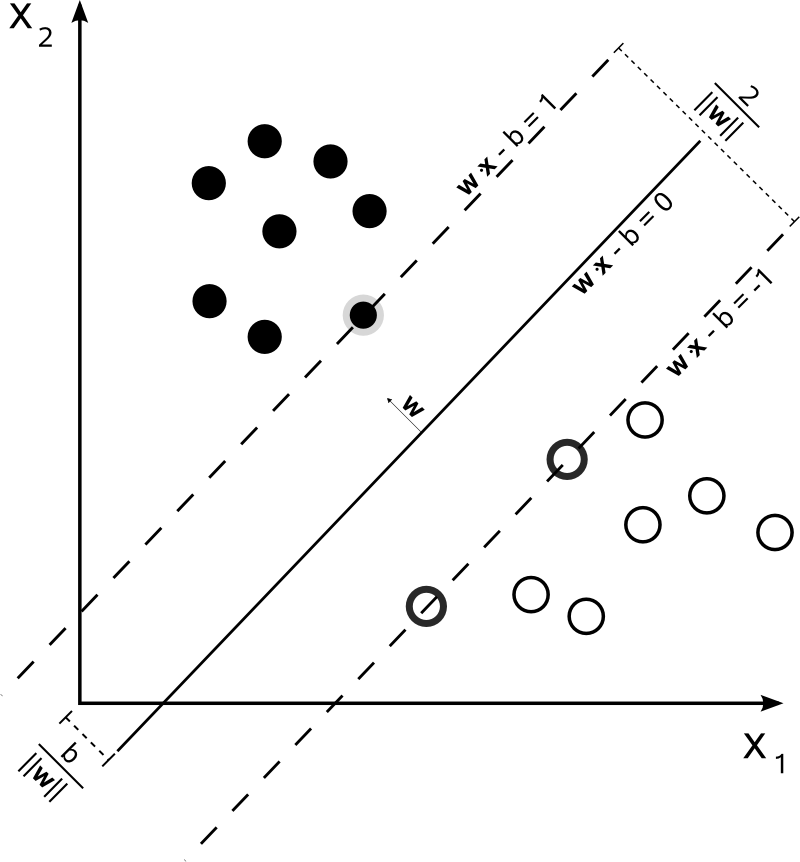
\includegraphics[width=.5\textwidth, keepaspectratio]{img/svm_max_sep_hyperplane.png}
\end{wrapfigure}

A hyperplane $h$ is given by a normal vector $\omega$ and a translation $b$ and the classification $h_{\omega, b}$ is defined as follows:
$$ h_{\omega, b}(x) = \text{sgn} (\omega^{T}x + b) \in \{-1, 1\}$$

We require that this evaluation coincides with the given classification of the points\footnote{
This may not always be possible.
In that unlucky case we require the condition for as many datapoints $x$ as possible and penalize misclassifications.}.


Additionally we require the parameter $\omega$ and $b$ to be such that no points lie in the \emph{margin} which is defined as the following set of points $x$\footnote{
It is easy to see that the width of the margin decreases when the length of $\omega$ increases.}:

$$ \left\{ x : \abs{h_{\omega,b} (x)} < 1 \right\} $$

We want to reduce the dimension of the original space and consider only a subset of features\footnote{
  This classification to be successful meaning that not all features are relevant.}.
In our model this implies that a certain fraction of weights is required to be zero resulting in a \emph{sparse classifier}.


A sparse classifier with sparsity $\rho$ is a linear classifier where a fraction of the $\omega$ entries is equal to 0:
$$ \rho(\omega) = \frac{\abs{\{ i \colon \omega_{i} = 0 \}}}{d} $$

Advantages of a sparse classifier are \emph{a smaller cost} of the classification and the fact that it results in a \emph{simpler model}\footnote{\emph{Occam's razor}: from a set of solutions to a problem select the one that makes the fewest assumptions.}

\section*{Material}

The sub directory \ttt{scip-workshop/support-vector-machine} is the place where you should place you python script.
It also contains a subdirectory \ttt{data}, which contains means to read in the data by the following python commands:

\lstset{language=python,%
basicstyle=\sffamily\footnotesize,%
numberstyle=\sffamily\tiny\color{siennabrown},stepnumber=1}
\begin{lstlisting}[frame=tb]{}
  from data.load_cancer import load_cancer

  dataset = load_cancer()
  X = np.array(dataset.data)
  y = np.array(dataset.targets)
\end{lstlisting}

The dataset is the classification of benign ($y=-1$) or malignant ($y=1$) breast cancer based on 30 features and contains 569 data points.
Out of these 212 are malignant and 357 are benign.
It is taken from:

\begin{center}
  \ttt{\small http://archive.ics.uci.edu/ml/machine-learning-databases/breast-cancer-wisconsin/}
\end{center}

For all the exercises you should split the dataset into two parts, one that you train on and one that you predict.

\section*{Exercise 1}

Your first task is to implement a linear svm with the following model.

Let the set of datapoints consist of $n$ $d$-dimensional features $X \in \R^{n,d}$, labeled by $y \in \{-1,+1\}^{n}$ and let $C > 0$ be a regularization parameter.
To penalize wrongly classified datapoints, consider as a loss function the \emph{Hinge loss}\footnote{
  Here $t$ is the evaluation of the classifier on datapoints.}:
$$l^{i}(t) :=  \max \{0, 1 - y^i t\} \text{\quad for } i \in \{1,\dots, n\}$$

As you want to minimize the penalty, and maximize the margin (equivalently minimize the length of $\omega$, since the width of the margin is given by $\frac{2}{\norm{\omega}}$), the model can now be written as the following optimization problem:

$$
\min\limits_{\omega, b}
\frac{C}{n} \sum\limits_{i = 1}^{n} l^i(\omega^{T}X^{i} + b)
+\frac{1}{2} \lVert \omega \rVert_{2}^{2}
$$

Substituting the Hinge loss for a variable

$$ \begin{aligned}
\xi^i &\geq l^i( \omega^T X^i + b ) \\
&= \max \{0, 1 - y^i (\omega^TX^i + b) \},
\end{aligned} $$

the above problem is equivalent to:

\begin{equation*}
\begin{array}{rll}
  \min\limits_{\omega, b}
  & \frac{C}{n} \sum\limits_{i = 1}^n \xi^i + \frac{1}{2} \lVert \omega \rVert_2^2
\\
  \text{such that}
  & 1 - y^i (\omega^T X^i +b) \leq \xi^i,
  & i \in \{1,\dots,n\}
\\
  & 0 \leq \xi^i,
  & i \in \{1,\dots, n\}
\end{array}
\end{equation*}

\section*{Exercise 2}

Modify the model from exercise 1 to produce a sparse classifier.

To implement a sparse classifier with sparsity $\rho$, add additional constraints and variables to the model\footnote{
  Another possibility would be to prefer sparse solutions using an $L1$-norm in the objective function.}.

\begin{equation*}
\begin{array}{rll}
  & \sum_{j \in d} v_{j} \leq \rho \cdot d
  &
\\
  & -B \cdot v_{j} \leq \omega_{j} \leq B \cdot v_{j},
  & j \in \{ 1, \dots, d \}
\\
  & v_{j} \in \{0,1\},
  & j \in \{1,\dots, d\}
\end{array}
\end{equation*}

For $i \in \{ 1, \dots, d \}$ assume the weights $\omega_j$ to be bounded by $-B$ and $B$ for a bound $B > 0$.
Only a fraction of these new binary indicator variables $v_j$ are allowed to be nonzero.
Then all the $v_j$ that are zero will force their corrensponding $\omega_j$ to be zero.

\section*{Exercise 3}

Depending on the number of positive and negative samples in the data we might want to weight the penalties differently, ensuring that points from one of the sets have a higher probability to be classified correctly\footnote{
  An application would be medical tests, where the a false negative should be highly unlikely, whereas a false positive is not disastrous.}.
This correction $c_i$ is applied in the objective function:

$$
\frac{C}{n} \sum\limits_{i = 1}^n c_i \xi^i + \frac{1}{2} \lVert \omega \rVert_2^2
\text{,\quad where } c_i =
\begin{cases}
  \alpha & \text{ if } y_i = 1 \\
  \beta & \text{ if } y_i = -1
\end{cases}
$$

Your task is to balance the data.

\end{document}

